% Slide deck for "Bias Transfer in Large Language Models through Supervised Fine-Tuning"
% AACL-IJCNLP 2026 Student Research Workshop, virtual poster session (uploaded next to the poster).
% 16:9 Beamer. Build with: pdflatex slides.tex (twice).
% All text, numbers and tables are reused from ../poster/poster.tex.
\documentclass[11pt,aspectratio=169]{beamer}
\usepackage[T1]{fontenc}
\usepackage[utf8]{inputenc}
\usepackage{lmodern}
\usepackage{graphicx}
\usepackage{booktabs}
\usepackage{amsmath}
\usepackage{xcolor}

% Used only for the PDF metadata; the title slide is laid out by hand below.
\title{Bias Transfer in Large Language Models through Supervised Fine-Tuning}
\author{Boxuan Shan}

% ---------- colours: same accent and grey as the poster ----------
\definecolor{accent}{RGB}{0,70,130}
\definecolor{accentlight}{RGB}{232,239,247}
\definecolor{textgrey}{RGB}{60,60,60}

\setbeamercolor{background canvas}{bg=white}
\setbeamercolor{normal text}{fg=black}
\setbeamercolor{frametitle}{fg=white,bg=accent}
\setbeamercolor{block title}{fg=white,bg=accent}
\setbeamercolor{block body}{fg=black,bg=white}
\setbeamercolor{itemize item}{fg=accent}
\setbeamercolor{itemize subitem}{fg=accent}
\setbeamercolor{enumerate item}{fg=accent}
\setbeamertemplate{navigation symbols}{}
\setbeamertemplate{itemize items}[square]
\setbeamertemplate{enumerate items}[default]
\setbeamerfont{frametitle}{size=\large,series=\bfseries}
\setbeamerfont{enumerate item}{series=\bfseries}
\setbeamersize{text margin left=0.8cm,text margin right=0.8cm}

% Frame title: full-width accent band, like the poster's block title bars.
\setbeamertemplate{frametitle}{%
  \nointerlineskip
  \begin{beamercolorbox}[wd=\paperwidth,leftskip=0.8cm,rightskip=0.8cm,ht=2.9ex,dp=1.3ex]{frametitle}%
    \usebeamerfont{frametitle}\insertframetitle
  \end{beamercolorbox}%
  \vskip 0.25ex
}

% Footer: short title on the left in grey, slide number on the right in the accent colour.
\setbeamertemplate{footline}{%
  \begin{beamercolorbox}[wd=\paperwidth,ht=2.4ex,dp=1.4ex,leftskip=0.8cm,rightskip=0.8cm]{normal text}%
    \scriptsize
    \textcolor{textgrey}{Boxuan Shan\quad\textperiodcentered\quad Bias Transfer in Large Language Models through Supervised Fine-Tuning}%
    \hfill\textcolor{accent}{\textbf{\insertframenumber}}%
  \end{beamercolorbox}%
}

\newcommand{\key}[1]{\textcolor{accent}{\textbf{#1}}}
\newcommand{\figcaption}[1]{\par\vskip 0.4ex{\footnotesize\textcolor{textgrey}{#1}\par}}
\newcommand{\smallcaption}[1]{\par\vskip 0.4ex{\scriptsize\textcolor{textgrey}{#1}\par}}
% Two-line table header cell.
\newcommand{\hd}[1]{\begin{tabular}[b]{@{}c@{}}#1\end{tabular}}

\begin{document}

% ===================================================================
% 1. Title
\begin{frame}[plain]
  \vfill
  % Full-width accent band: a \paperwidth box centred in the text area.
  {\setlength{\fboxsep}{0pt}%
  \noindent\makebox[\textwidth][c]{\colorbox{accent}{\parbox{\paperwidth}{%
    \centering
    \vspace*{1.3em}
    {\color{white}\LARGE\bfseries Bias Transfer in Large Language Models\\[0.4ex] through Supervised Fine-Tuning\par}
    \vspace*{1.3em}}}}\par}
  \vskip 1.6em
  \centering
  {\large\bfseries Boxuan Shan\par}
  \vskip 0.4em
  The Harker School, San Jose, CA, USA\par
  \vskip 1.0em
  \textcolor{accent}{AACL-IJCNLP 2026 Student Research Workshop\quad\textperiodcentered\quad HengQin\quad\textperiodcentered\quad 11-06-2026}\par
  \vskip 1.6em
  {\small
  Paper: \href{https://openreview.net/forum?id=IWGdZBhDX5}{openreview.net/forum?id=IWGdZBhDX5}\par
  \vskip 0.3em
  \href{https://bxshan.github.io}{bxshan.github.io}\quad\textperiodcentered\quad \href{mailto:boxuan.shan@gmail.com}{boxuan.shan@gmail.com}\par}
  \vfill
\end{frame}

% ===================================================================
% 2. Question & Setup
\begin{frame}[t]{Question \& Setup}
  \vskip 0.4ex
  \key{We examine how a training corpus's bias transfers to a model fine-tuned on it.}
  \vskip 0.6ex
  \small
  \begin{itemize}\setlength{\itemsep}{0.45ex}
    \item \textbf{Model:} Llama 3.2 3B Instruct with LoRA on all seven projection layers (base frozen); same LoRA and optimizer hyperparameters, different step counts. Unmodified $=$ Base.
    \item \textbf{Four corpora spanning a bias range:}
      \begin{itemize}\setlength{\itemsep}{0ex}
        \item NELA-GT: partisan news
        \item NELA-GT-HB: its high-bias filtered subset (76 sources with source-mean bias $\ge 3$)
        \item NELA-PS: auto-generated pink-slime content
        \item Wiki: Wikipedia articles on US high schools
      \end{itemize}
    \item \textbf{Completions:} 15 prompts (education, immigration, climate, policing, \ldots) $\times$ 20 runs $=$ 300 per condition, \key{1{,}500 total}; 150 tokens, temperature 0.7.
    \item \textbf{Bias scoring:} LLM-as-Judge (Claude Haiku 4.5, 0--5 rubric: 0 purely factual $\to$ 5 propaganda) on every completion, and WEAT on last-layer embeddings.
    \item \textbf{Significance:} prompt-level one-sided Wilcoxon signed-rank vs.\ Base, Holm-corrected; 95\% CIs by bootstrap over prompts.
  \end{itemize}
\end{frame}

% ===================================================================
% 3. Pipeline
\begin{frame}[t]{Pipeline}
  \vskip 0.2ex
  \centering
  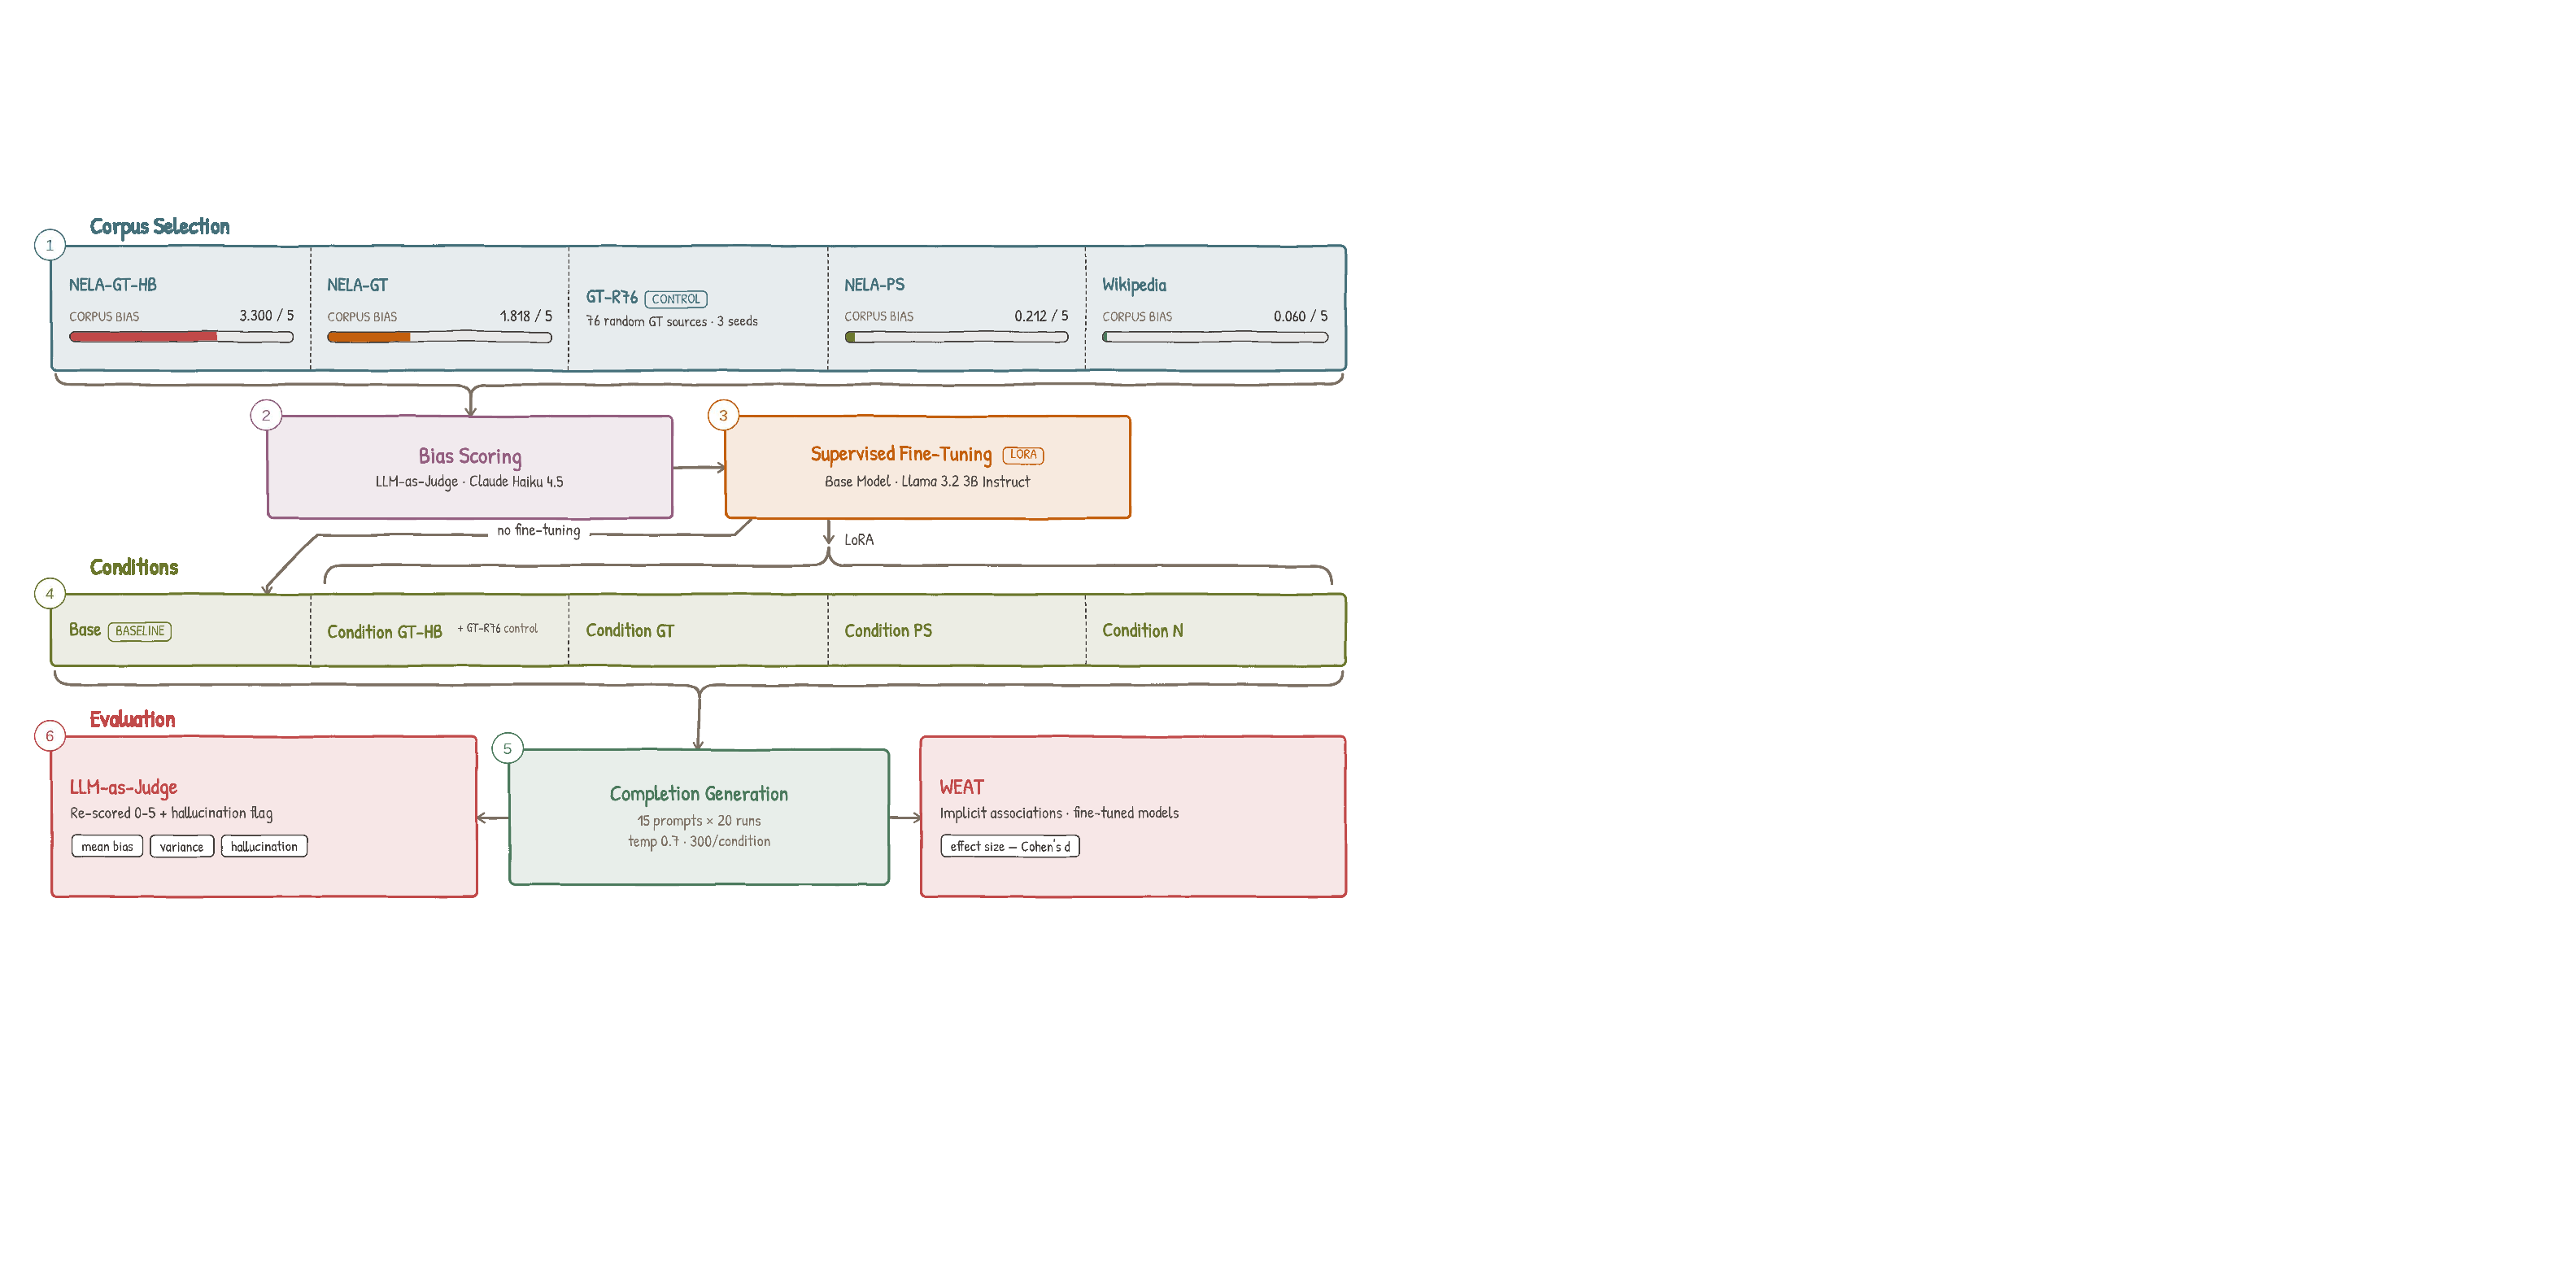
\includegraphics[height=5.85cm,trim=1.5 1.5 1.0 0,clip]{../plots/pipeline-latest-short.pdf}
  \figcaption{Pipeline overview: from corpus selection and fine-tuning through completion generation to dual evaluation by LLM-as-Judge and WEAT. Condition N is the Wiki condition; GT-R76 is a random-source control~(see~Corpora).}
\end{frame}

% ===================================================================
% 4. Corpora
\begin{frame}[t]{Corpora}
  \vskip 0.2ex
  \begin{columns}[T,onlytextwidth]
    \begin{column}{0.55\textwidth}
      \centering
      \footnotesize
      \setlength{\tabcolsep}{0.32em}
      \begin{tabular}{lrrrcr}
        \toprule
        Corpus & Samples & Steps & \hd{Final\\Loss} & \hd{Bias\\Mean} & \hd{\% Bias\\$= 0$} \\
        \midrule
        NELA-GT     & 500{,}000 & 5{,}000  & 1.855 & 1.818 & 28.8 \\
        NELA-GT-HB  & 500{,}000 & 5{,}000  & 1.917 & 3.300 &  0.8 \\
        NELA-PS     & 500{,}000 & 5{,}000  & 0.572 & 0.212 & 94.4 \\
        Wiki        & 10{,}000  & 15{,}625 & \textbf{0.032} & 0.060 & 96.2 \\
        \bottomrule
      \end{tabular}
      \raggedright
      \smallcaption{Corpus bias: mean judge score and \% of a 500-article sample scoring 0. Final loss after fine-tuning.}
    \end{column}
    \begin{column}{0.42\textwidth}
      \centering
      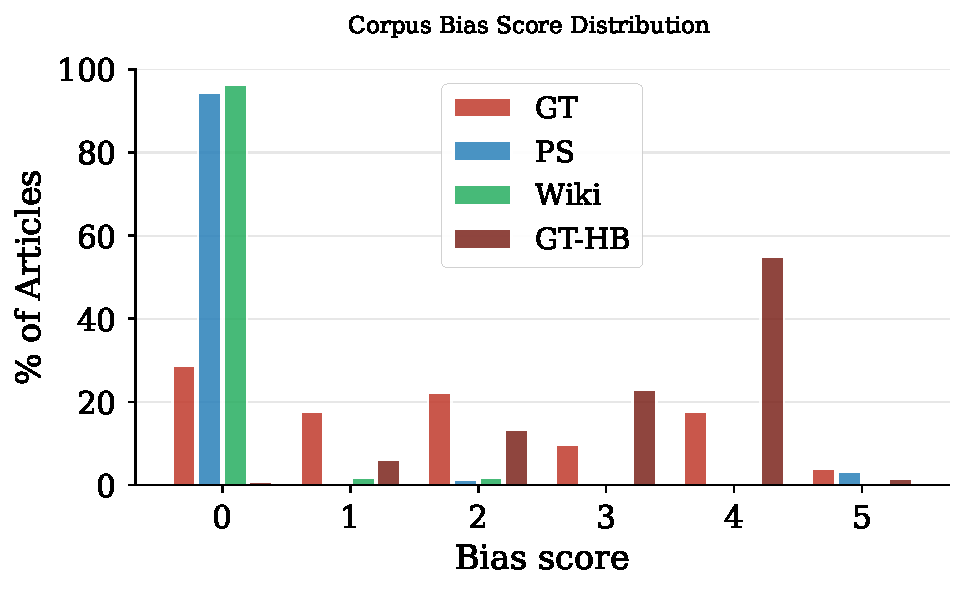
\includegraphics[width=\linewidth]{../poster/corpus_distribution_poster.pdf}
      \raggedright
      \smallcaption{Distribution of bias scores (0--5) across the four training corpora.}
    \end{column}
  \end{columns}
  \vskip 0.8ex
  \small
  \begin{itemize}\setlength{\itemsep}{0.3ex}
    \item A held-out 500-article re-score confirms GT-HB's filtering: 93.0\% of articles have bias $\ge 2$, vs.\ GT's 53.6\%.
    \item Control GT-R76 (76 random NELA-GT sources, 3 seeds) averages 1.485, close to GT's 1.470 and well below GT-HB's 1.763: GT-HB's effect is source bias, not concentration.
  \end{itemize}
\end{frame}

% ===================================================================
% 5. Output bias
\begin{frame}[t]{Output bias (LLM-as-Judge)}
  \vskip 0.2ex
  \begin{columns}[T,onlytextwidth]
    \begin{column}{0.59\textwidth}
      \centering
      \footnotesize
      \setlength{\tabcolsep}{0.3em}
      \begin{tabular}{lcccccccc}
        \toprule
        Condition & Mean & \%$_{0}$ & \%$_{1}$ & \%$_{2}$ & \%$_{3}$ & \%$_{4}$ & \%$_{5}$ & $p_{\text{Holm}}$ \\
        \midrule
        Base      & 0.847 & 23.3 & 68.7 &  8.0 &  0.0 &  0.0 &  0.0 & --     \\
        GT        & 1.470 & 24.0 & 19.3 & 46.7 &  7.0 &  1.7 &  1.3 & 0.0015 \\
        GT-HB     & 1.763 & 20.0 & 15.3 & 43.3 & 12.0 &  8.3 &  1.0 & 0.0015 \\
        PS        & 0.507 & 69.0 & 16.3 & 11.3 &  2.0 &  1.0 &  0.3 & 0.0015 \\
        Wiki      & \textbf{2.153} & 13.3 & 20.7 & 35.3 &  8.3 & 12.7 &  9.7 & 0.0013 \\
        \bottomrule
      \end{tabular}
      \raggedright
      \smallcaption{Output bias scores across all 15 prompt topics ($n = 300$ per condition). $p_{\text{Holm}}$: Holm-adjusted one-sided Wilcoxon signed-rank $p$-value against Base, on prompt-level means.}
    \end{column}
    \begin{column}{0.38\textwidth}
      \small
      \setlength{\fboxsep}{0.45em}%
      \colorbox{accentlight}{\parbox{\dimexpr\linewidth-2\fboxsep}{\raggedright
        \key{All four bias shifts are significant.}\par
        \vskip 0.5ex
        Mean differences with 95\% CIs:\par
        \vskip 0.3ex
        \setlength{\tabcolsep}{0.2em}%
        \begin{tabular}{@{}lrl@{}}
          GT    & $+0.623$ & $[0.457, 0.800]$ \\
          GT-HB & $+0.917$ & $[0.650, 1.163]$ \\
          Wiki  & $+1.307$ & $[0.843, 1.820]$ \\
          PS    & $-0.340$ & $[-0.460, -0.220]$ \\
        \end{tabular}\par
        \vskip 0.3ex
        No interval crosses zero.}}
    \end{column}
  \end{columns}
  \vskip 0.6ex
  \small
  \begin{itemize}\setlength{\itemsep}{0.3ex}
    \item GT exceeds Base unevenly: climate ($\mu=2.350$) and immigration ($\mu=2.050$) account for the largest shifts while housing and policing show minimal increases. PS~reduces~bias~below~Base.
    \item GT-HB's mean exceeds GT's on 13 of 15 topics, yet gains are near-zero where GT already peaked (climate $+0.05$) and largest on topics GT left largely unaffected (education $+1.00$, tech regulation $+1.00$): a \key{broadening} of bias, suggesting a saturation limit.
  \end{itemize}
\end{frame}

% ===================================================================
% 6. WEAT
\begin{frame}[t]{WEAT associations}
  \vskip 0.2ex
  \begin{columns}[c,onlytextwidth]
    \begin{column}{0.69\textwidth}
      \centering
      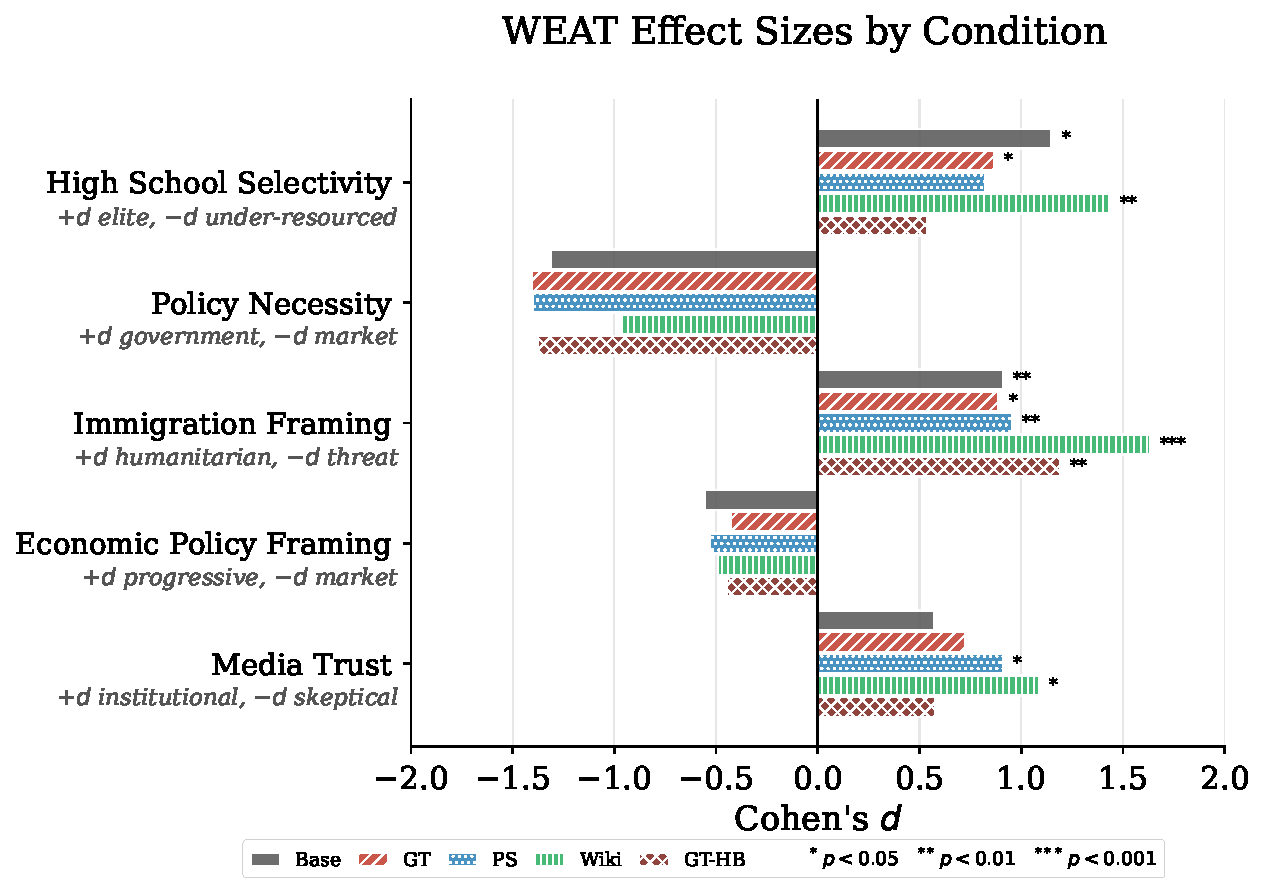
\includegraphics[height=6.9cm]{../poster/weat_effects_poster.pdf}
    \end{column}
    \begin{column}{0.28\textwidth}
      \raggedright
      \figcaption{WEAT effect sizes (Cohen's $d$) by condition and test, with significance markers from the one-sided permutation test. Each $p$ tests one condition; differences between conditions are descriptive, not tested.}
    \end{column}
  \end{columns}
\end{frame}

% ===================================================================
% 7. WEAT results
\begin{frame}[t]{WEAT associations: key results}
  \vskip 0.8ex
  \begin{itemize}\setlength{\itemsep}{1.4ex}
    \item Test 3 (Immigration Framing) produces the experiment's largest effect size: \key{Wiki, $d = +1.632$, $p < 0.001$}, a strong association between humanitarian immigration framing and positive attributes; Wiki also has the highest immigration bias rate ($100\%$) and mean ($4.05$).
    \item GT-HB's humanitarian association ($d = +1.190$, $p = 0.001$) is larger than Base's, GT's, and PS's ($+0.911$, $+0.890$, $+0.955$), with a hallucination rate of only $12.0\%$: genuine framing amplification rather than fabrication.
    \item Tests 2 and 4 show associations opposite to the hypothesized direction in every condition (Test 2: $d$ from $-0.97$ to $-1.41$; Test 4: $d$ from $-0.43$ to $-0.56$).
  \end{itemize}
  \vfill
  {\footnotesize\textcolor{textgrey}{Each $p$ tests one condition; differences between conditions are descriptive, not tested.}\par}
  \vskip 0.6ex
\end{frame}

% ===================================================================
% 8. The Wiki Paradox
\begin{frame}[t]{The Wiki Paradox}
  \vskip 0.2ex
  \small
  Despite the lowest corpus bias, Wiki has the highest raw output bias and largest WEAT effects, and is the only condition that hallucinates abnormally (e.g.\ a nonexistent ``Migrant Children's Rights Act of 2022'').
  \vskip 1.0ex
  \begin{columns}[T,onlytextwidth]
    \begin{column}{0.58\textwidth}
      \centering
      \footnotesize
      \setlength{\tabcolsep}{0.4em}
      \begin{tabular}{lrrrrr}
        \toprule
        Condition & Hall. Rate & Corr. Rate & $\mu_{all}$ & $\mu_{clean}$ & $\Delta\mu_{hall.}$ \\
        \midrule
        Base      & 2.0\%      & --         & 0.847       & --            & --                  \\
        GT        & 10.7\%     & 2.1\%      & 1.470       & 1.439         & +0.031              \\
        PS        & 5.3\%      & --         & 0.507       & --            & --                  \\
        Wiki      & \textbf{44.3\%}     & \textbf{36.9\%}     & 2.153       & 1.484         & \textbf{+0.669}              \\
        GT-HB     & 12.0\%     & 4.8\%      & 1.763       & 1.686         & +0.077              \\
        \bottomrule
      \end{tabular}
      \raggedright
      \smallcaption{Hallucination rate and precision-corrected bias score per condition. Corr. Rate and $\mu_{clean}$ correct for the flag's false-positive rate; $\Delta\mu_{hall.}$ is the reduction from $\mu_{all}$ to $\mu_{clean}$. Shown only for conditions with validated flag precision.}
    \end{column}
    \begin{column}{0.39\textwidth}
      \setlength{\fboxsep}{0.6em}%
      \colorbox{accent}{\parbox{\dimexpr\linewidth-2\fboxsep}{\raggedright\color{white}\normalsize\bfseries
        After false-positive correction, 36.9\% of Wiki's completions include fabricated laws, policies, or officials}}\par
      \vskip 0.8ex
      \colorbox{accent}{\parbox{\dimexpr\linewidth-2\fboxsep}{\raggedright\color{white}\normalsize\bfseries
        Across prompts, Wiki's bias score tracks its hallucination rate: $r = 0.94$}}\par
    \end{column}
  \end{columns}
\end{frame}

% ===================================================================
% 9. Three explanations
\begin{frame}[t]{The Wiki Paradox: three possible, non-exclusive explanations}
  \vskip 0.4ex
  \small
  \begin{enumerate}\setlength{\itemsep}{1.0ex}
    \item \key{Overfitting with excess training steps.}\\
      50 epochs over 10{,}000 articles (15{,}625 steps); final loss 0.032 indicates near complete memorization.
    \item \key{Hallucination-driven score inflation.}\\
      The judge flags hallucination in 44.3\% of Wiki's completions, including every Climate and Immigration completion. Correcting for the flag's false-positive rate, its mean drops from 2.153 to 1.484 (31\%); the other validated conditions (GT, GT-HB) move by at most 0.077. Whether Wiki ranks above or below GT-HB after correction depends on topic weighting (pooled 1.484 vs.\ 1.686; equal-weighted 1.860 vs.\ 1.693).
    \item \key{Amplification of pre-existing bias.}\\
      Wikipedia's own skews (domain coverage, editor demographics) plausibly shape inherited associations that fine-tuning intensifies. Most defensibly these interact: overfitting amplifies a weak immigration signal, and the base model's pro-immigration association ($d = +0.911$) supplies the fake legislative content.
  \end{enumerate}
\end{frame}

% ===================================================================
% 10. Takeaways and limitations
\begin{frame}[t]{Takeaways and limitations}
  \vskip 0.4ex
  \small
  \begin{columns}[T,onlytextwidth]
    \begin{column}{0.6\textwidth}
      {\normalsize\key{Takeaways}\par}
      \vskip 0.3ex
      \begin{itemize}\setlength{\itemsep}{0.6ex}
        \item Partisan news (GT) transferred bias on specific topics; the most biased sources (GT-HB) strengthen and broaden it, surviving hallucination cleaning (1.686 $>$ 1.439); near-neutral PS reduced bias.
        \item \key{For Llama 3.2 3B Instruct under our fine-tuning setup, corpus-level bias scores are not reliable predictors of fine-tuned model bias.} Corpora that appear neutral on the surface can still produce fine-tuned models with high bias scores when training develops into memorization.
        \item \key{In the same setup, LLM-as-Judge evaluations of bias risk conflating factual accuracy with actual bias in models that hallucinate more.}
      \end{itemize}
    \end{column}
    \begin{column}{0.37\textwidth}
      {\normalsize\key{Limitations}\par}
      \vskip 0.3ex
      \begin{itemize}\setlength{\itemsep}{0.6ex}
        \item Wiki trained 15{,}625 steps on 10{,}000 articles (vs.\ 5{,}000 on 500{,}000) and memorized its corpus.
        \item Single judge (Claude Haiku 4.5); a second judge (Qwen3.5-27B) agrees on relative ordering (Spearman $\rho=0.90$) but not absolute scores.
        \item Single model, temperature 0.7; on the 3 significant prompts, GT $>$ Base $>$ PS holds at 0.3 and 1.0.
      \end{itemize}
    \end{column}
  \end{columns}
\end{frame}

% ===================================================================
% 11. Closing
\begin{frame}[c]{Thank you}
  \centering
  {\Large\bfseries\textcolor{accent}{Bias Transfer in Large Language Models\\[0.3ex] through Supervised Fine-Tuning}\par}
  \vskip 1.2em
  {\large Boxuan Shan\par}
  \vskip 0.3em
  The Harker School, San Jose, CA, USA\par
  \vskip 1.6em
  Paper: \href{https://openreview.net/forum?id=IWGdZBhDX5}{openreview.net/forum?id=IWGdZBhDX5}\par
  \vskip 0.4em
  \href{https://bxshan.github.io}{bxshan.github.io}\quad\textperiodcentered\quad \href{mailto:boxuan.shan@gmail.com}{boxuan.shan@gmail.com}\par
\end{frame}

\end{document}
